\documentclass[a4paper,11pt,dvipdfmx]{ujarticle}
% パッケージ
\usepackage{graphicx}
\usepackage{url}
% レイアウト指定を記述したファイルの読み込み
\input{layout}

% タイトルと氏名を変更せよ.
\title{日本におけるデジタル化の現状}
\author{G584242025 宇津翔大}

\begin{document}

\maketitle %ここにタイトルが入る

% ここから本文
\section{ブロードバンドの整備状況}% 節見出し: \section{}
% を使う

OECDによるブロードバンド回線の普及に関する調査% 本文(1)
\cite{oecd}によると、%  参考文献の参照: \cite{}
図\ref{fig:myfig}%  図番号の参照: \ref{}
に示すように、日本における100人あたりの光ファイバー回線の加入者数は29.0で、韓国、スウェーデン、ノルウェーに続いて第
4位になっている。% を使う
% 文献データベースのキーワードは oecd と imd
% になっている.

% 図の挿入
% \includegraphics{}
% を
\begin{figure}[htbp]% \begin{figure}[htbp]
\centering% \end{figure}
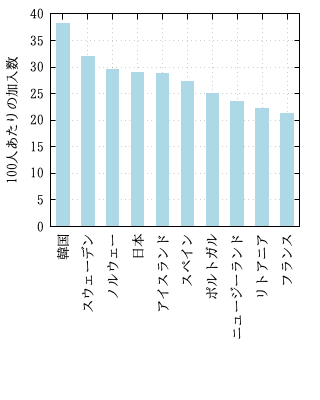
\includegraphics{fig11.png}% で囲み
\caption{光ファイバー回線の加入者数(100人あたり}\label{fig:myfig}% \caption{}
\end{figure}% で図のタイトルを入れる.
% \label{}
% を使って図番号が参照できるようにする
% また,
% \centering
% で図が中央に来るようにする

% ーーー
\section{デジタル競争力ランキング}% 節見出し(2)

国際経営開発研究所(IMD)の調査\cite{imd}によると、表\ref{tbl:mytbl}に示すように、日本のデジタル競争力のランキ
ングは調査対象の64カ国中、総合で28位、知識分野で25位となっている。% 本文(2)

\begin{table}[htbp]
    \centering
    \caption{デジタル競争力ランキング(64カ国中}\label{tbl:mytbl}% 表の挿入
\begin{tabular}{|c|c|c|}
    \hline
    国&総合&知識\\
    \hline
    米国&1位&3位\\
    \hline
    香港&2位&5位\\
    \hline
    スウェーデン&3位&2位\\
    \hline
    デンマーク&3位&2位\\
    \hline
    シンガポール&5位&4位\\
    \hline
    \hline
    韓国&12位&15位\\
    \hline
    中国&15位&6位\\
    \hline
    \hline
    日本&28位&25位\\
    \hline
\end{tabular}
\end{table}
    % \begin{tabular}
% \end{tabular}    
% による表の記述を 
% \begin{table}[htbp]
% \end{table}
% で囲み
% \caption{}
% で表のタイトルを入れる.
% \label{}
% を使って表番号が参照できるようにする
% また,
% \centering
% で表が中央に来るようにする

% ーーー
\section{考察}% 見出し(3)
\begin{itemize}% 考察
\item 光ファイバーの普及状況とデジタル競争力に相関性はない
\item デジタル競争力は知識分野で総合ランキングまで決まるわけではない%
\end{itemize}% \begin{itemize}
% \end{itemize}
% を使って箇条書きで記述する

% ここに参考文献が入る
%
\bibliographystyle{junsrt}
\bibliography{exercise.bib}

\end{document}